\chapter{SMALL/THINGS} 
\label{sec:smallthings}
\lstset{style=6502Style}

In this book we have looked at lots of different elements of \textit{Uridium's} graphics and gameplay. We
have spent a lot of time in the weeds and pixels and assembly and learnt almost everything there is that is
interesting to know about how the game was accomplished. But we have not developed a sense of the structure
of the game's source code. We will remedy that now. We ought to come away from this book with a basic sense of how much code
and data the game contains and what are the features that dominate the game binary's 47,000 bytes. 

Maybe we should
pause and reflect on that number first: the game binary is made up of just over 47,000 bytes. To get a sense of how
tiny this number is in the context of modern computing, all of \textit{Uridium} would fit more than 233 million times over into the storage
of a mass-market personal computer in 2026.
\footnote{Assuming a capacity of 1 Terabyte, which is over 1 trillion bytes (1,099,511,627,776 to be exact).}
The fact that it was possible to achieve so much with so little is 
one of the great achievements of the era of 8-bit computing in which Andrew Braybrook created \textit{Uridium}.

What is even more remarkable is how little of the 47,000 or so bytes is accounted for by the assembly code that we
have devoted so much attention to in this book. The engine that runs the game and manages every element of its display
and mechanics is a mere 4000 bytes or so. Into this tiny space every flourish and every nuance in gameplay and design
has been compacted and squashed. What is going on in the remaining 43,000 bytes you might wonder. Overleaf we have a diagram
that endeavours to show you. Each major component of the games source code is represented in the order in which it appears in the game
binary. Each
component is represented as a dreadnought whose relative size to the others tells you how much of the source code it takes up.

\clearpage
\vspace{0.5cm}
\begin{figure}[H]
 \hspace{0.45cm}
 \begin{adjustbox}{width=16cm,left}
   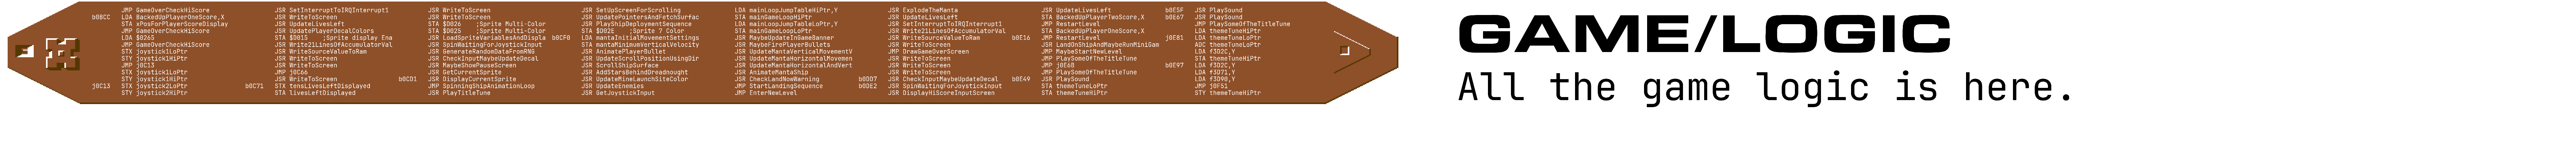
\includegraphics{src/source_map/game_logic.png}
 \end{adjustbox}
\end{figure}
\vspace{-0.3cm}

\begin{figure}[H]
 \hspace{0.45cm}
 \begin{adjustbox}{width=16cm,left}
   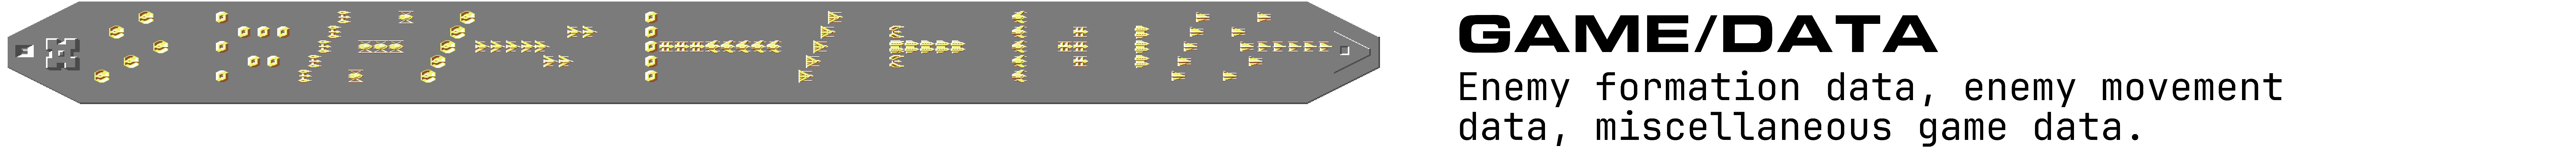
\includegraphics{src/source_map/game_data.png}
 \end{adjustbox}
\end{figure}
\vspace{-0.3cm}

\begin{figure}[H]
 \hspace{0.45cm}
 \begin{adjustbox}{width=16cm,left}
   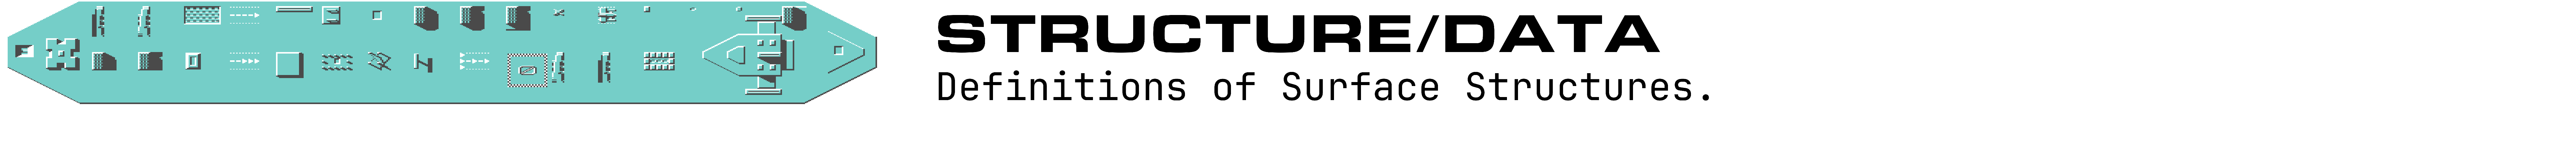
\includegraphics{src/source_map/structure_data.png}
 \end{adjustbox}
\end{figure}
\vspace{-0.3cm}

\begin{figure}[H]
  \hspace{0.45cm}
 \begin{adjustbox}{width=16cm,left}
   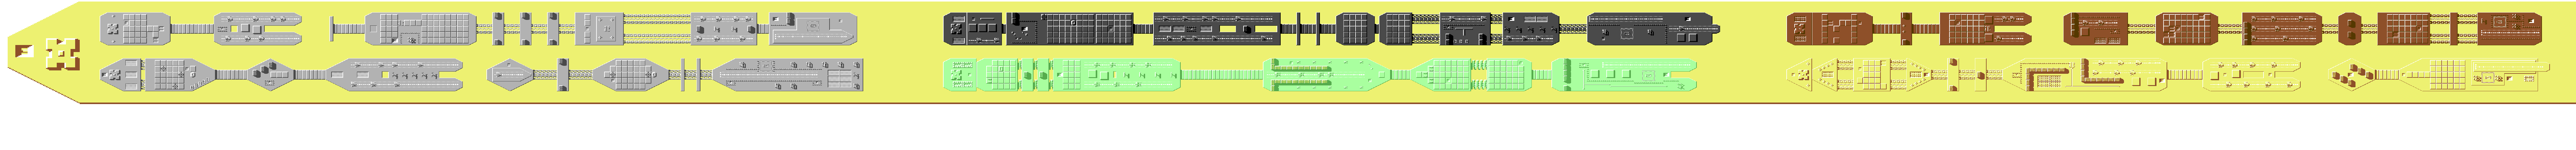
\includegraphics{src/source_map/level_data_1.png}
 \end{adjustbox}
\end{figure}
\vspace{-0.3cm}

\begin{figure}[H]
 \hspace{0.45cm}
 \begin{adjustbox}{width=16cm,left}
   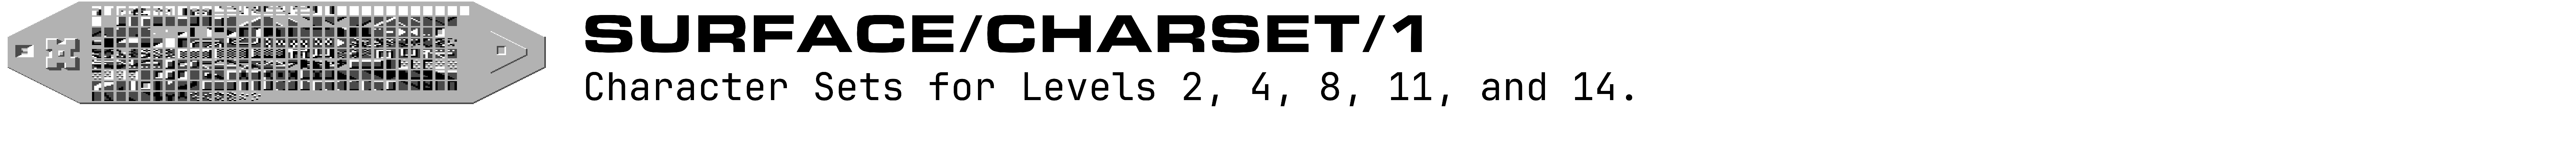
\includegraphics{src/source_map/surface_charset_1.png}
 \end{adjustbox}
\end{figure}
\vspace{-0.3cm}

\begin{figure}[H]
 \hspace{0.45cm}
 \begin{adjustbox}{width=16cm,left}
   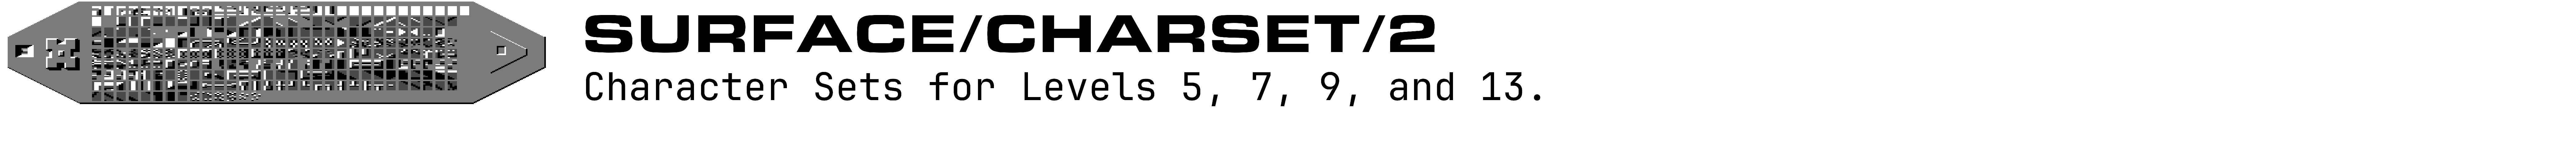
\includegraphics{src/source_map/surface_charset_2.png}
 \end{adjustbox}
\end{figure}
\vspace{-0.3cm}

\begin{figure}[H]
 \hspace{0.45cm}
 \begin{adjustbox}{width=16cm,left}
   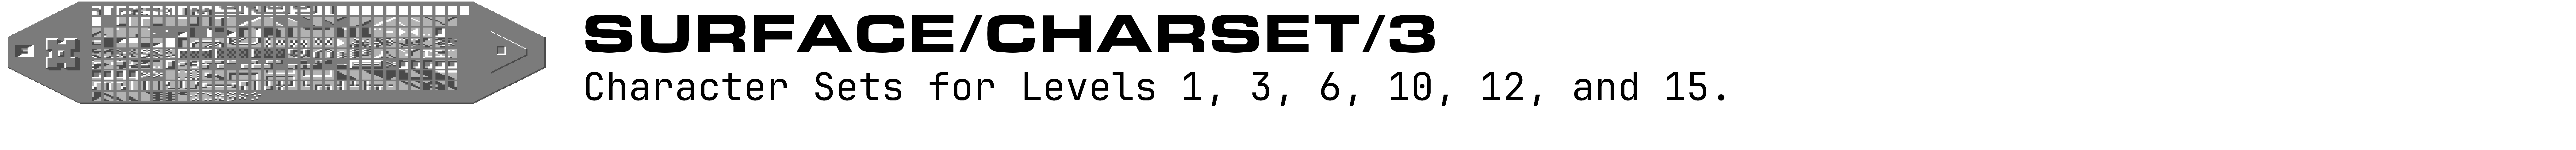
\includegraphics{src/source_map/surface_charset_3.png}
 \end{adjustbox}
\end{figure}
\vspace{-0.3cm}

\begin{figure}[H]
 \hspace{0.45cm}
 \begin{adjustbox}{width=16cm,left}
   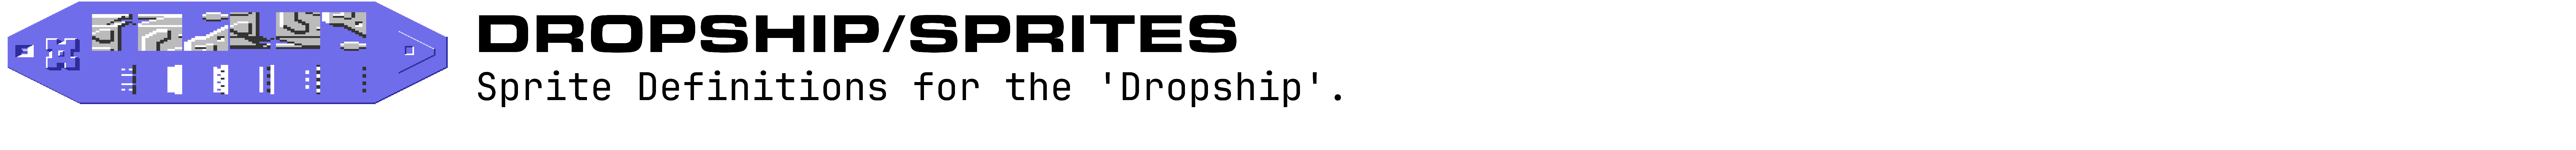
\includegraphics{src/source_map/dropship_sprites.png}
 \end{adjustbox}
\end{figure}
\vspace{-0.3cm}

\begin{figure}[H]
 \hspace{0.45cm}
 \begin{adjustbox}{width=16cm,left}
   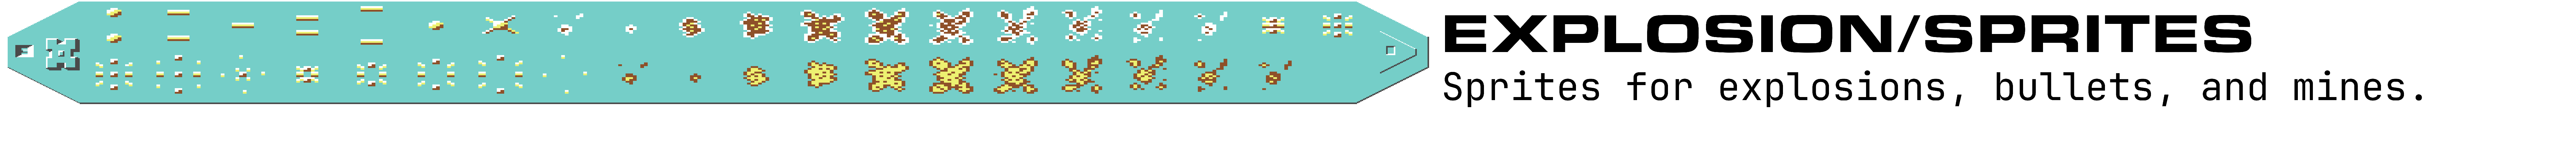
\includegraphics{src/source_map/explosion_sprites.png}
 \end{adjustbox}
\end{figure}
\vspace{-0.3cm}

\begin{figure}[H]
 \hspace{0.45cm}
 \begin{adjustbox}{width=16cm,left}
   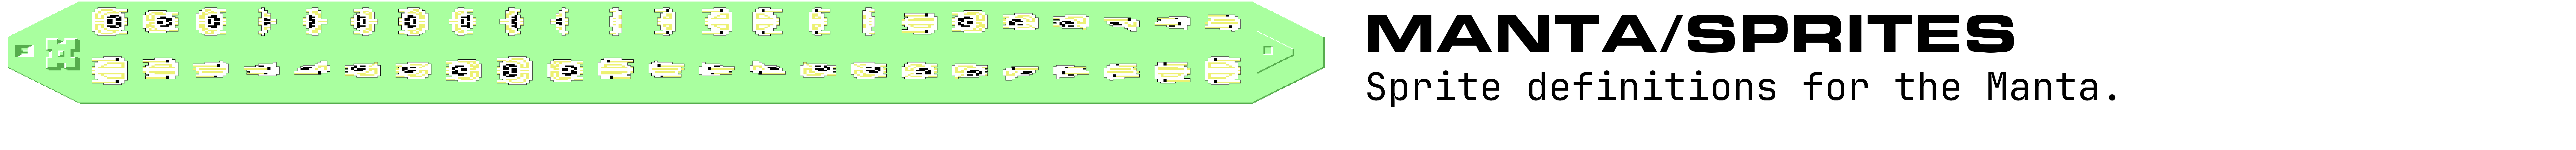
\includegraphics{src/source_map/manta_sprites.png}
 \end{adjustbox}
\end{figure}
\vspace{-0.3cm}

\begin{figure}[H]
 \hspace{0.45cm}
 \begin{adjustbox}{width=16cm,left}
   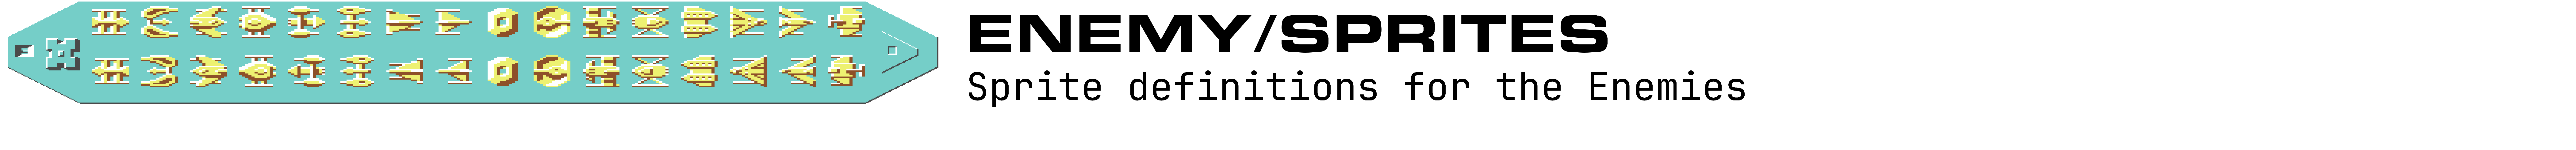
\includegraphics{src/source_map/enemy_sprites.png}
 \end{adjustbox}
\end{figure}
\vspace{-0.3cm}

\begin{figure}[H]
 \hspace{0.45cm}
 \begin{adjustbox}{width=16cm,left}
   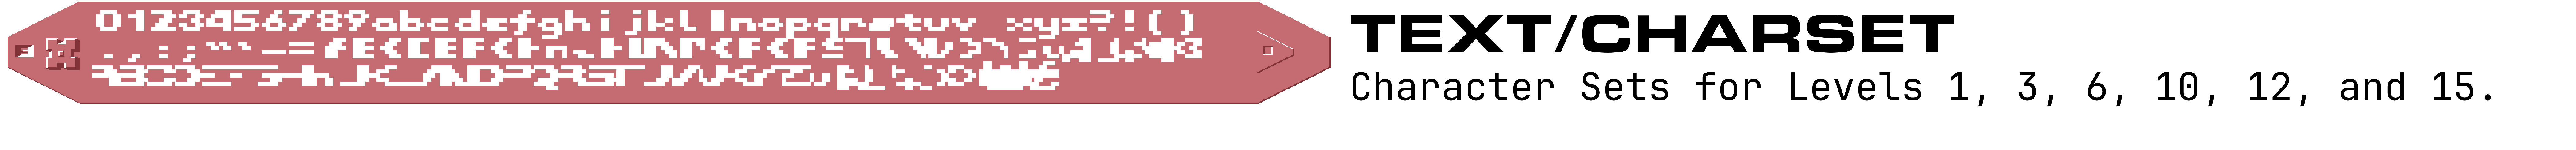
\includegraphics{src/source_map/text_charset.png}
 \end{adjustbox}
\end{figure}
\clearpage
What is immediately obvious in the diagram opposite is that we don't have enough room on the page
for the level data and that it has to spill over onto this one. This level data consists of the definitions
for the level dreadnoughts we looked at in the   
\hyperref[sec:surface]{{\textbf{\euro{SUR/FACES}}}}
chapter. But even this data by itself isn't enough to create a level dreadnought, it relies on each of the
\euro{SURFACE/CHARSET} sections below it to provide the tiles for the surfaces and on the \euro{STRUCTURE/DATA} above it to provide
definitions for each of the strips and structures that we covered in the
\hyperref[sec:structure]{{\textbf{\euro{STRUC/TURE}}}}
chapter.

The result is that just over 13,000 bytes are dedicated to defining the game's levels, over 4 times the amount of space
devoted to the core game logic in \euro{GAME/LOGIC}.

\begin{figure}[H]
\vspace{-0.05cm}
 \hspace{-2.60cm}
 \begin{adjustbox}{width=16cm,left}
   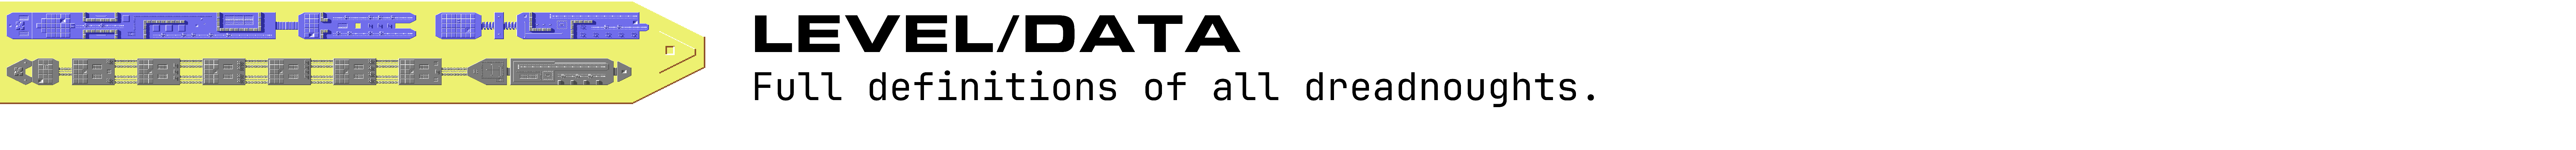
\includegraphics{src/source_map/level_data_2.png}
 \end{adjustbox}
\end{figure}
\vspace{-0.6cm}

Only slightly behind the level data lies the space devoted to sprites, which clocks in at just over 9,000 bytes. Of the four different
types of sprites to which the game devotes precious real estate, the sprites devoted to all manner of bullets and explosions
(\euro{EXPLOSION/SPRITES})
have a narrow lead on the rest of the pack. The quantity is understandable given the variety of effects involved, which we covered in the
\hyperref[sec:explosions]{\euro{EX/PLODE}}
chapter. 

What the diagram opposite really brings home is the sheer quantity of available space devoted to different aspects of the player's Manta.
We explored some of these in the 
\hyperref[sec:ships]{\euro{MANTA/SPIN}}
and
\hyperref[sec:flip]{\euro{MANTA/FLIP}}
chapters. It really brings home the amount of effort and detail the game devotes to rendering the manta as realistically and compellingly 
as possible.

Now that we appreciate how much of the game is given over to the data that supports the graphics and how little, at least relatively speaking,
is dedicated the assembly code that runs the game itself it is worth digging further into the \euro{GAME/LOGIC} segment opposite to see
what is is made up of. We want to answer the question: how much code does each element of the game take up? In the diagrams below we break
out the sections of the \euro{GAME/LOGIC} in the order in which they appear in the disassembled source code. 

The first section of the code is occupied, perhaps naturally enough, with displaying the games title sequence. This includes the title screen
and the scrolling banner. This sequence runs in a loop until the player presses fire to commence a game. It makes use of the 
\euro{DEMO/MODE} section which we find further down.

\begin{figure}[H]
   \begin{adjustbox}{width=16cm,left}
        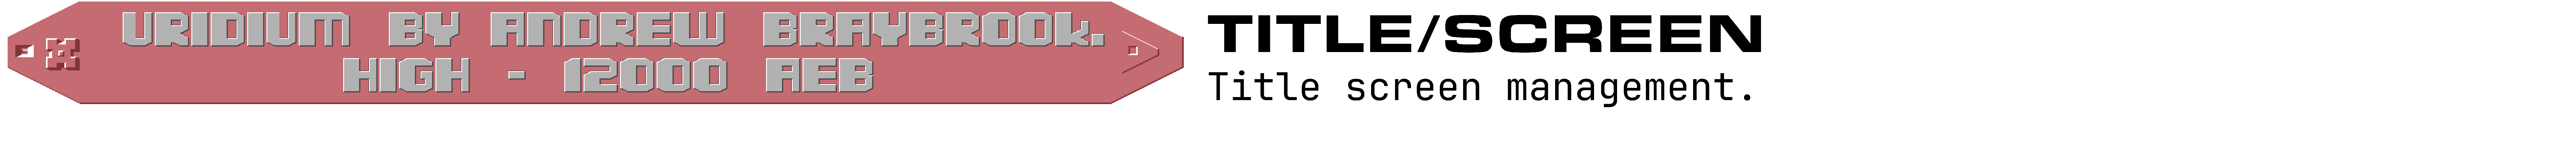
\includegraphics{src/game_logic/1_title_screen.png}
         \end{adjustbox}
\end{figure}
\vspace{-0.6cm}

Immediately after this section we find the code that manages the spinning manta seen in the leve-entry sequence, which we covered in 
\hyperref[sec:ships]{\euro{MANTA/SPIN}}.

\begin{figure}[H]
   \begin{adjustbox}{width=16cm,left}
        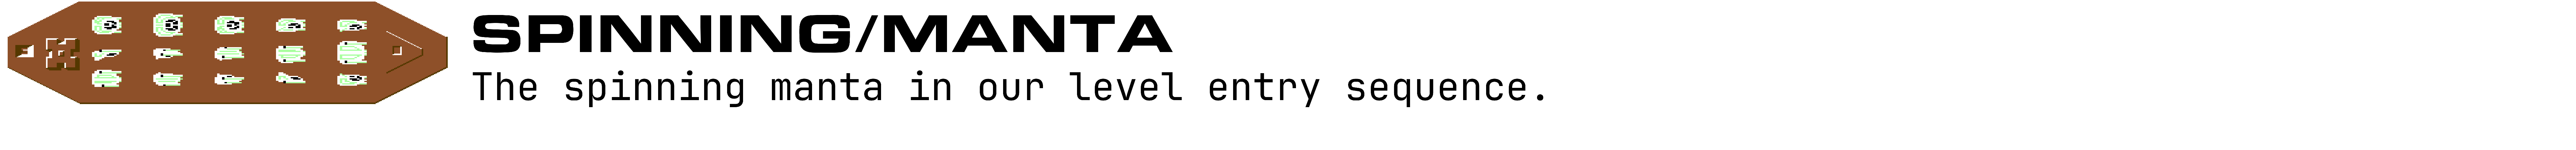
\includegraphics{src/game_logic/2_spinning_manta.png}
         \end{adjustbox}
\end{figure}
\vspace{-0.5cm}

\begin{figure}[H]
   \begin{adjustbox}{width=16cm,left}
        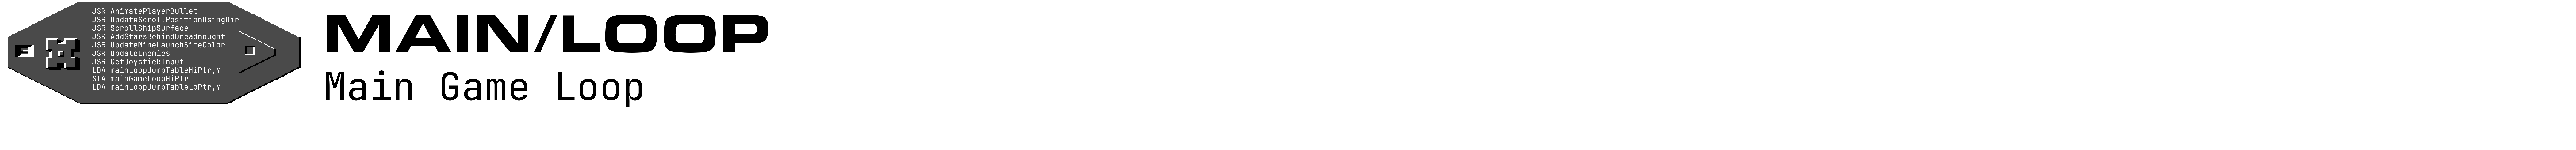
\includegraphics{src/game_logic/3_main_loop.png}
         \end{adjustbox}
\end{figure}
\vspace{-0.5cm}

\begin{figure}[H]
   \begin{adjustbox}{width=16cm,left}
        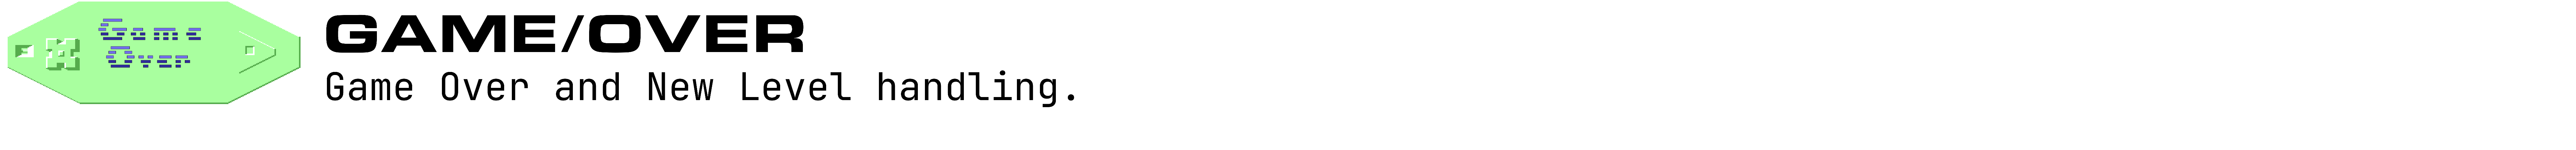
\includegraphics{src/game_logic/4_game_over.png}
         \end{adjustbox}
\end{figure}
\vspace{-0.5cm}

\begin{figure}[H]
   \begin{adjustbox}{width=16cm,left}
        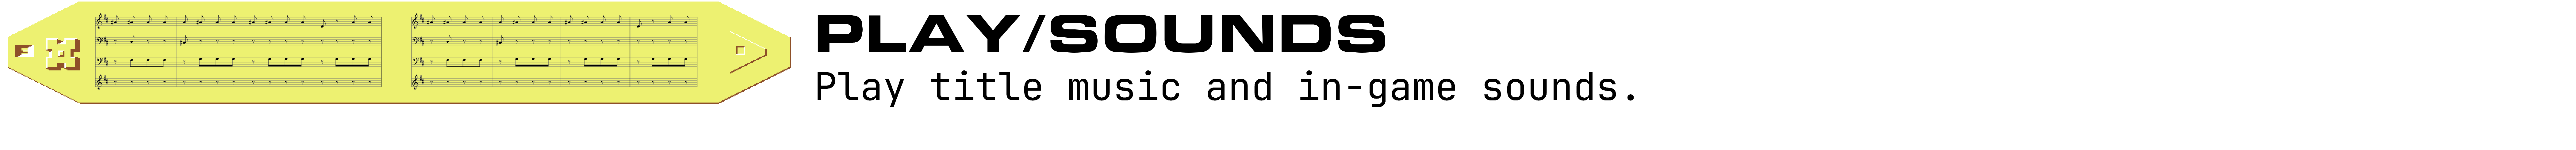
\includegraphics{src/game_logic/5_play_sounds.png}
         \end{adjustbox}
\end{figure}
\vspace{-0.5cm}

\begin{figure}[H]
   \begin{adjustbox}{width=16cm,left}
        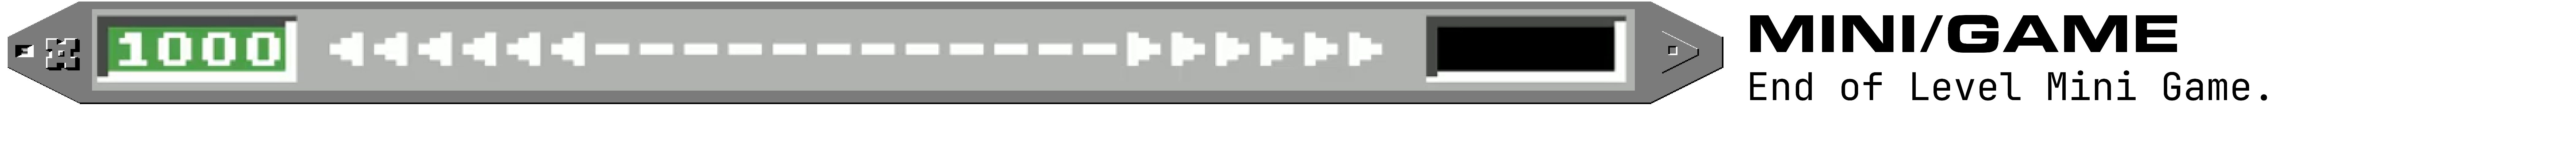
\includegraphics{src/game_logic/6_mini_game.png}
         \end{adjustbox}
\end{figure}
\vspace{-0.5cm}

\begin{figure}[H]
   \begin{adjustbox}{width=16cm,left}
        
\includegraphics{src/game_logic/7_destruct_sequence.png}
         \end{adjustbox}
\end{figure}
\vspace{-0.5cm}

\begin{figure}[H]
   \begin{adjustbox}{width=16cm,left}
        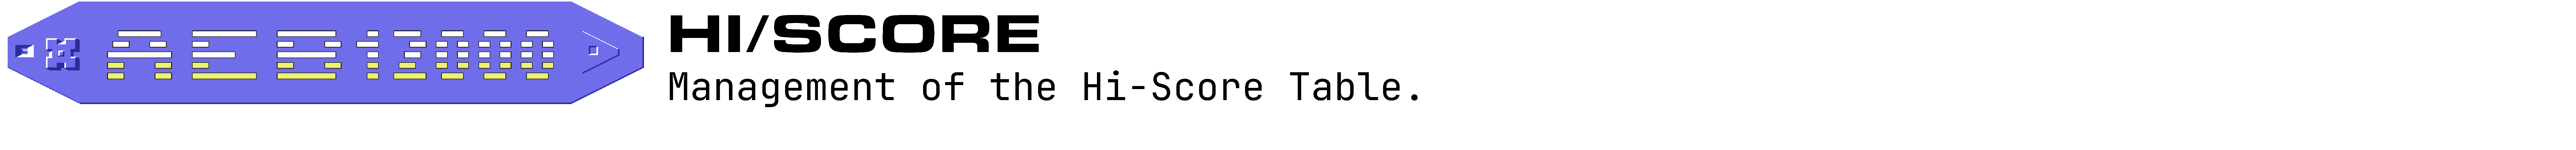
\includegraphics{src/game_logic/8_hi_score.png}
         \end{adjustbox}
\end{figure}
\vspace{-0.5cm}

\begin{figure}[H]
   \begin{adjustbox}{width=16cm,left}
        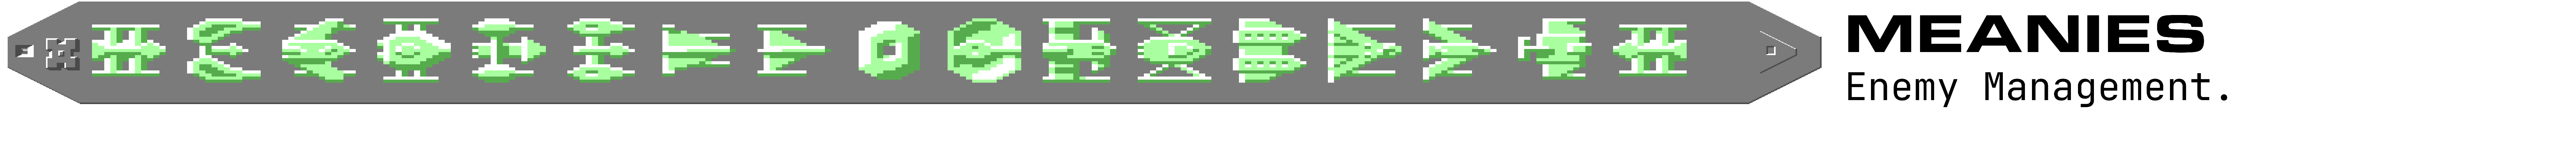
\includegraphics{src/game_logic/9_enemy_management.png}
         \end{adjustbox}
\end{figure}
\vspace{-0.5cm}

\begin{figure}[H]
   \begin{adjustbox}{width=16cm,left}
        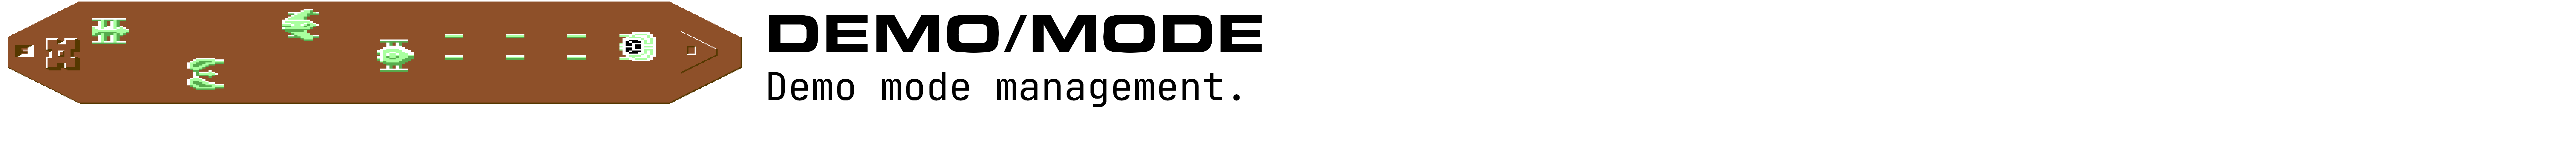
\includegraphics{src/game_logic/10_demo_mode.png}
         \end{adjustbox}
\end{figure}
\vspace{-0.5cm}

\begin{figure}[H]
   \begin{adjustbox}{width=16cm,left}
        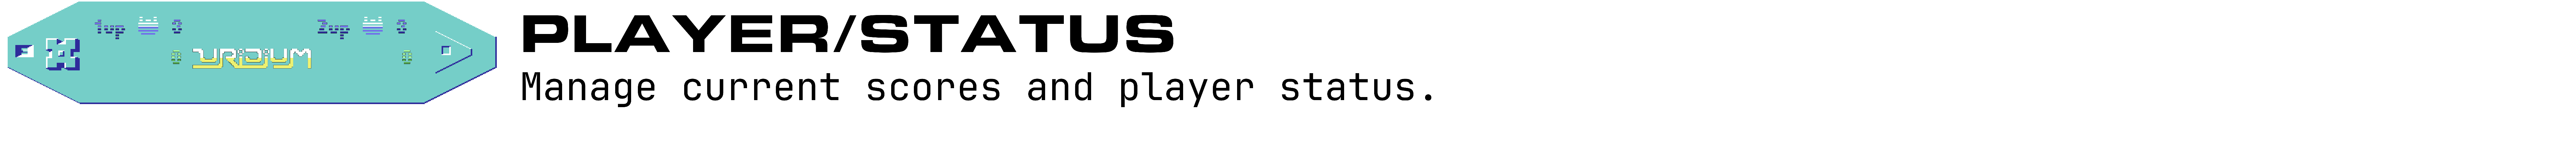
\includegraphics{src/game_logic/11_in_game.png}
         \end{adjustbox}
\end{figure}
\vspace{-0.5cm}

\begin{figure}[H]
   \begin{adjustbox}{width=16cm,left}
        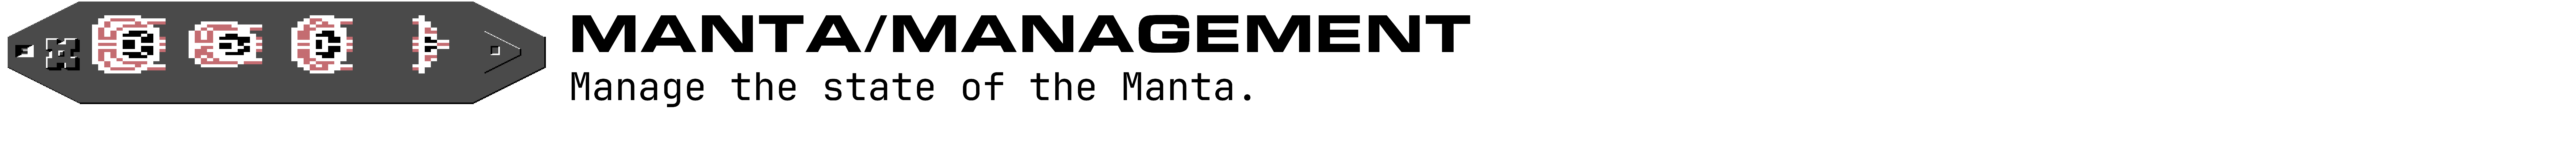
\includegraphics{src/game_logic/12_manta_state.png}
         \end{adjustbox}
\end{figure}
\vspace{-0.5cm}

\begin{figure}[H]
   \begin{adjustbox}{width=16cm,left}
        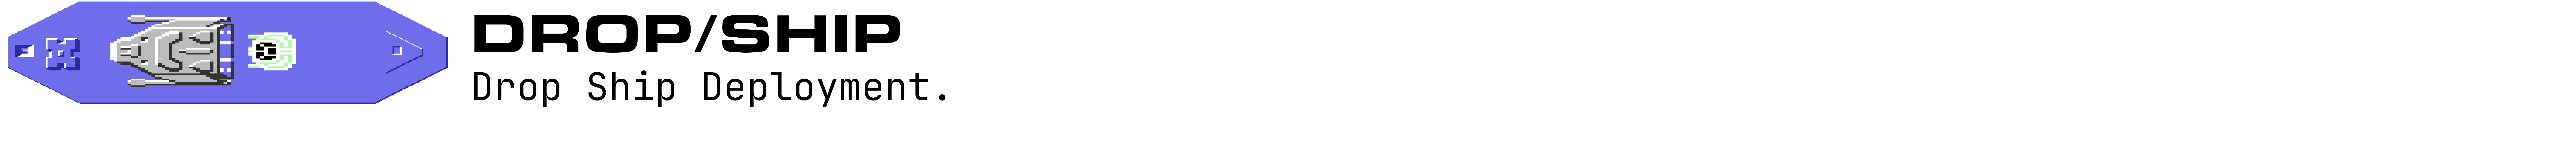
\includegraphics{src/game_logic/13_drop_ship_deployment.png}
         \end{adjustbox}
\end{figure}
\vspace{-0.5cm}

\begin{figure}[H]
   \begin{adjustbox}{width=16cm,left}
        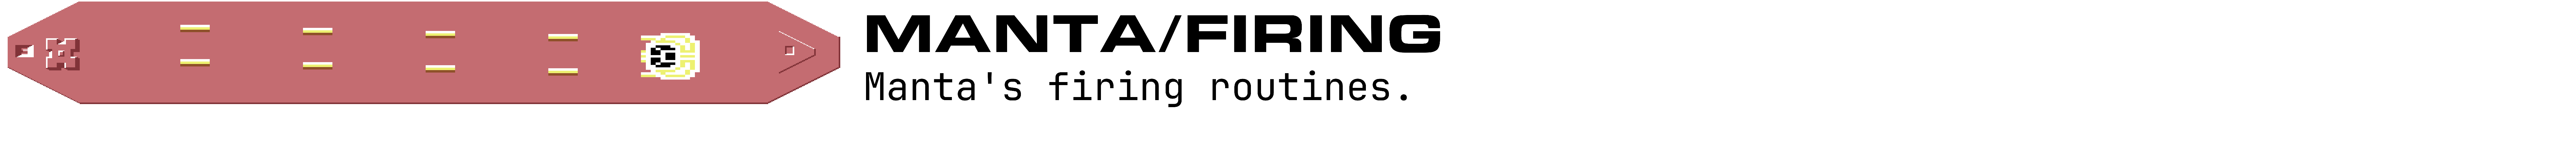
\includegraphics{src/game_logic/14_manta_firing.png}
         \end{adjustbox}
\end{figure}
\vspace{-0.5cm}

\begin{figure}[H]
   \begin{adjustbox}{width=16cm,left}
        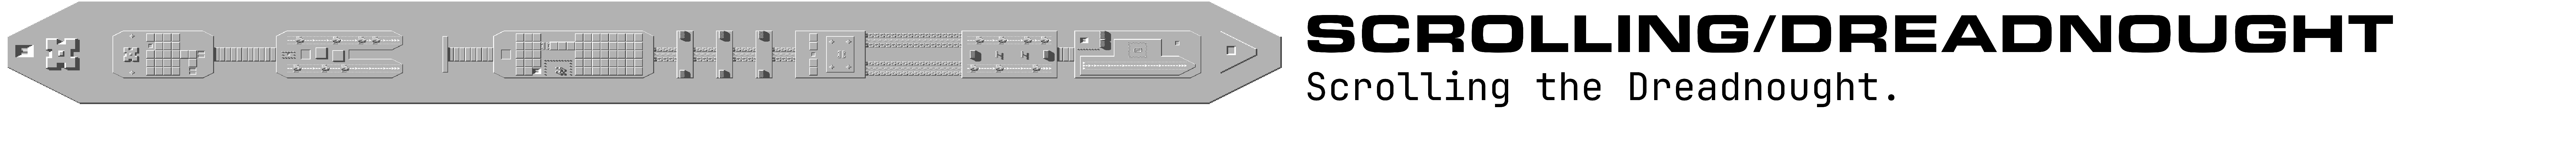
\includegraphics{src/game_logic/15_scrolling_dreadnought.png}
         \end{adjustbox}
\end{figure}
\vspace{-0.5cm}
\clearpage

Next up is the game's \euro{MAIN/LOOP}. This is a tight section of 40 or so lines that acts as the nerve centre
of the game while it is in play. We get a better sense of the relative scale if we reproduce this main loop
in full below. You can see how short it is, this gives you an idea of the relative length of the other
sections of code in the diagram opposite.

\begin{lstlisting}[basicstyle=\scriptsize\ttfamily]
MainGameLoop
  LDA shouldWaitUntilReady       ; Wait for any interrupt to finish.
  BNE MainGameLoop               ; Keep waiting until ready.

  JSR AnimatePlayerBullet        ; Animate any player bullets.
  JSR UpdateScrollPosition       ; Update our scroll position.
  JSR ScrollShipSurface          ; Scroll the ship's surface.
  JSR AddStarsBehindDreadnought  ; Add stars behind the dreadnought.
  JSR UpdateMineLaunchSiteColor  ; Flash the colour of visible mine sites.
  JSR UpdateEnemies              ; Update enemy positions.
  INC indexToJumpTable           ; Increment index to jump table.
  JSR GetJoystickInput           ; Get player input.

  ; Perform one of seven functions at each loop.
  LDA indexToJumpTable           ; Load the jump table index.
  AND #$07                       ; Clamp it to between 0 and 7.
  TAY                            ; Put it in the Y register.
  LDA mainLoopJumpTableHiPtr,Y   ; Use it to get the high byte of the routine.
  STA mainGameLoopHiPtr          ; Store it in the 2nd byte of the JSR stmt below.
  LDA mainLoopJumpTableLoPtr,Y   ; Use index to get the low byte of routine.
  STA mainGameLoopLoPtr          ; Store it in the 1st byte of hte JSR stmt below.
mainGameLoopLoPtr   =*+$01       ; The first byte of the address to JSR below.
mainGameLoopHiPtr   =*+$02       ; The second byte of the address to JSR below.
  JSR MaybeUpdateInGameBanner    ; Run the routine selected by the index.

  JSR MaybeFirePlayerBullets     ; Fire any new player bullets.
  JSR UpdateMantaVerticalMovementVelocity      ; Update vertical player movement.
  JSR UpdateMantaHorizontalMovementVelocity    ; Update horizontal movement.
  JSR UpdateMantaHorizontalAndVerticalPosition ; Update manta's position.
  JSR AnimateMantaShip           ; Animate the movement of the manta.
  JSR CheckLandNowWarning        ; Display land now warning if necessary.
  LDA landNowActivated           ; Check if land now activated.
  BPL ResumeLoop                 ; If not, loop again.
  JMP StartLandingSequence       ; Otherwise, start landing sequence.

ResumeLoop
  LDA hasMantaBeenHit            ; Check if manta has been hit.
  BEQ MainGameLoop               ; If not, loop again.
\end{lstlisting}

A casual glance at our diagram reveals that two elements in particular dominate the game's assembly code real-estate. These are the code devoted to the mini-game, where the player
earns extra points at the end of each level, and the code concerned with management of the player's enemies. We devoted four separate sections
to the enemy behaviour, from 
\hyperref[sec:meanies]{\euro{57/MEANIES}}
to
\hyperref[sec:meanie_fire]{\euro{MEANIE/FIRE}}
so it is not such a surprise to find so much space consumed with managing their antics. Of course, we haven't covered the behaviour and detail
of the mini-game at all in this little book. This is for the very personal reason that I don't find it interesting, so I couldn't really bring
myself to spend any time on it. 

You might spot other elements that I haven't covered in the book, some of these will be remedied over time. But it is clear as we look
closer that considerable space is given over to details of the manta, such as general management in \euro{MANTA/MANAGEMENT}, firing bullets
in \euro{MANTA/FIRING}, as well as the \euro{DROP/SHIP} sequence. We can also see that the scrolling mechanism which we covered in 
\hyperref[sec:scrolling]{\euro{SKIP/SCROLL}} is behind only the mini-game and enemy management in the amount of code it requires.

